
\documentclass[mcs]{scsthesis}
\usepackage{url}
\usepackage{amsmath}
\usepackage{amsthm}
\usepackage{graphicx}

\title {Biased Nearest Neighbour Search}
\author {Daniel Minor}
\thesissupervisor {Patrick Morin}
\director {Douglas Howe}

\begin{document}

\newtheorem*{thm}{Theorem}[section]

\beforepreface

\prefacesection

\chapter*{Abstract}

TODO:

\chapter*{Acknowledgements}

TODO:

\afterpreface

\chapter{Introduction}

\section{Problem Statement}

We investigate the utility of data structures for biased nearest neighbour
search in practice. The nearest neighbour search problem is to return the
closest point in a set of points to a specified query point. In the biased 
variant of this problem, it is assumed that information is available which
allows for more common queries to be answered more quickly.

Nearest neighbour search is of considerable practical interest with
applications in geographical information systems, computer graphics,
computer vision, signal processing and machine learning.

Nearest neighbour search has received a large amount of attention from both
theoretical and applied computer scientists since the early 1970s. It is an
example of a problem which suffers from the so-called "curse of
dimensionality" where as the number of dimensions increases, an increasingly
large number of points must be searched until performance in practice is no
better than a brute force search of all of the points. Even in low dimensions,
nearest neighbour search can be a difficult problem in practice given a large
enough point set or the requirement to support a large number of queries in a
timely fashion.

Due to both the number of practical applications and to the fact that it suffers
from the curse of dimensionality, a large number of heuristic solutions as well
as more rigouressly defined data structures and algorithms have been proposed
for use in solving nearest neighbour search problems.

Recently, two groups of researchers \cite{chan} \cite{oddson} have proposed a
a biased data structure, called odds-on trees in \cite{oddson},  which can be
applied to a variety of geometrical search problems and which seems as though it
may be of practical as well as theoretical interest.

A distribution sensitive data structure makes use of knowledge of the
probability distribution of the queries in order to answer queries with an
expected runtime which is of the order of the entropy, or amount of randomness,
present in the query distribution. 

In a sense, the odds-on tree data structure provides a theoretical basis for
the creation of heuristics to accelerate geometrical search problems. Since
nearest neighbour search is a problem of practical interest with a number of
existing heuristic solutions with varying degrees of justification in theory,
it seemed a natural area to which to apply the odds-on tree with a view to
determining its effectiveness in practice.

Our goal is to implement a practical data structure based on the theoretical
results about odds-on trees.  This involves design and implementation work as
well as extensive experimentation to establish correctness and performance
characteristics.  Since the performance of odds-on trees is by design
dependent upon the probability distribution of the queries, it is necessary
to do experimentation based upon a wide variety of query distributions,
including some derived from applications of nearest neighbour search.

\section{Definitions}

TODO:

Query point: A point for which a nearest neighbour should be found. 

Site: a potential nearest neighbour.

Metric

\(L^2\) metric.

Comparison Tree model

Planar subdivision

\section{Results Summary}

TODO:

\section{Organization of the Thesis}

The remainder of the thesis is organized as follows: Chapter 2 summarizes
previous work for biased search, distribution sensitive data structures and
nearest neighbour search.  Chapter 3 describes the design and implementation of
the odds-on tree, including an description of alternative designs which were
explored.  Chapter 4 gives details on the experimentation performed and results
obtained, and Chapter 5 summarizes the results and discusses potential 
future work.

\chapter{Previous Work}

In this section we examine previous work relevant to odds-on tree. In the first
section we examine data structures for nearest-neighbour search. In the second
section we present results on biased search in one dimension and describe
the odds-on tree data structure.

\section{Nearest Neighbour Search}

In this section we examine data structures and algorithms for nearest-neighbour
search. We restrict ourselves to algorithms which work in a comparison tree
model, where data structures perform comparisons on coordinates.

TODO: better definition of comparison trees

Since they are not relevant for the remainder of this thesis, we do not consider
approaches based upon hashing, such as locality sensitive hashing or so-called
metric trees, where points are sorted based upon distance to a reference
point rather than based upon their coordinates. Locality sensitive hashing and
several different metric trees are described and evaluated experimentally in
\cite{practicalann}.

We also restrict ourselves to an in-memory model, and so do not consider
external memory based data structures such as R-trees \cite{rtree}. Since an
odds-on tree is essentially a cache, it does not make sense to consider an
external memory representation, although an odds-on tree may be quite useful
as an in-memory cache for an external memory data structure. 

\subsection{Voronoi Diagrams}

One way of looking at nearest neighbour search is as a subdivision of the plane
into disjoint areas based upon which site to which they are closest. Finding
the nearest neighbour to a query point is then a matter of determining which
subdivision the query point lies in.

A traditional name for this problem is the post-office problem, where given a
set of sites (the post-offices) determine for a given query point which
post-office is closest \cite{dutch}.

The Voronoi diagram is a data structure containing an explicit subdivision of
the plane based upon which site is closest, according to a specified metric. A
Voronoi diagram divides the plane (or hyper-plane) into disjoint areas called
Voronoi cells. For the \(L^2\) metric, these cells will be convex.

\begin{thm} \emph{(Voronoi Diagram Construction)}
The Voronoi diagram for a set of n points in two dimensions can be computed
in time \(O(n log n)\). In higher dimensions, the time becomes
\(O(n log n + n^\ceil(d/2))\) where d is the dimensionality of the space.
\cite{dutch}.
\end{thm}

TODO: insert voronoi diagram

\subsubsection{Nearest Neighbour Search in a Voronoi Diagram}

Once the Voronoi diagram is constructed, determining the nearest neighbour can
be done by performing point location to determine in which Voronoi cell the
query point lies.

In 2D, an efficient data structure for the more general problem of point
location in a planar subdivision was described by Kirkpatrick
\cite{kirkpatrick}. It based upon first triangulating the subdivision and then
removing independent vertices (those which do not share an edge) from the
triangulation to create a triangulation with fewer faces. Provided a constant
number of vertices are removed from the triangulation at each step, performing
the triangulation recursively will result in a data structure which supports
point location in logarithmic time.

\begin{thm} \emph{(Point Location in the Plane)}
A data structure exists using \(O(n)\) storage which allows for planar
point location to be performed in \(O(log n)\) time \cite{kirkpatrick}.
\end{thm}

In higher dimensions, it is possible to solve this problem 

TODO: description of Chazelle's algorithm.

\begin{thm} \emph{(Point Location in Higher Dimensions)}
A data structure exists using \(O(n^d)\) storage which allows for  
point location in a d-dimensional arrangment of hyperplanes to be performed in
\(O(log n)\) time \cite{chazelle}.
\end{thm}

Nearest-neigbhour search can be performed using Voronoi diagrams and provides
efficient algorithms in the plane. To extend this to reporting k-nearest
neighbours, once the Voronoi cell containting the query point has been
identified, the neighbour cells of the Voronoi diagram can be examined until
a sufficient number of neighbours has been found. 

In higher dimensions, the time requirement to build a Voronoi diagram and the
space requirement for the point location data structure both depend upon the
dimension of the space in an exponential fasion, which limits both their
theoretical and practical utility for this problem.

\subsection{Quadtrees}

Quadtrees are based upon recursively dividing n-dimensional space into \(2^n\)
equal sized hypercubes, with each node in the tree keeping pointers to its
children.  In the two dimensional case, this means that space is divided into
four quadrants, hence the name quadtrees. Quadtrees were introduced in 1974 by
Finkel and Bentley \cite{quadtree}. 

In this thesis, we only use quadtrees which are derived from an underlying point
set.  In this case, the recursive sub-division is done until each hypercube
contains a single point from the point set.

The root of the quadtree is the hypercube containing all of the points, a leaf
is a hypercube containing a single point, and the height of a quadtree
is the longest path from the root of the quadtree to the leaf of a quadtree
\cite{dutch}.

\begin{thm} \emph{(Height of a Quadtree)}
The height of a quadtree for a set of n points has an upper bound of \(log(s/c)
+ 3/2\), where c is the smallest distance between any two points in the set, and
s is the side length of the initial square containing all of the points.
\cite{dutch}.
\end{thm}

Note that the height of the quadtree is not bounded by n.

\begin{thm} \emph{(Quadtree Construction)}
A quadtree of height h containing n points can be constructed in \(O((h + 1)n)\)
time \cite{dutch}.
\end{thm}

\subsubsection{Point Location in a Quadtree}

Point location in a quadtree is performed by recursively visiting nodes
starting with the root node. At each step, the child node containing the query
point is visited, and the algorithm terminates when a leaf node is reached.

\begin{thm} \emph{(Point Location in a Quadtree)} 
Point location in a quadtree of height h can be performed in time \(O(h)\). 
\end{thm}

\subsubsection{Nearest Neighbour Search in a Quadtree}

Given a query point p the quadtree node containing p, if any, can be found by
starting at the root, comparing p to the bounds of the each child of the root,
and recursively visiting the child containing p until a leaf node is found.  
Since the maximum depth of a quadtree with n points is not bounded by n, the
running time of this search algorithm is also not bounded by n. This search,
along with a means of performing region queries was described in
\cite{quadtree}.

To perform nearest neighbour search in a quadtree we adapt the procedure given
in \cite{samet} for kd-trees. Finding a nearest neighbour in a quadtree is done
by maintaining a priority queue of nodes to visit, which initially contains the
root node. The algorithm proceeds by removing a node from the priority queue and
examining each of its children. If the child node contains a point it is added
to the result set.

Otherwise, the distance from the query point to each child node is calculated
and if it is smaller than the distance to the current furthest result point,
it is added to the priority queue. The work done by this algorithm is at
least the same amount of work required to do perform a point location query.

\begin{thm} \emph{(Nearest Neighbour Search in a Quadtree)} 
Nearest neighbour search in a quadtree of height h requires \(O(h)\) time.
\end{thm}

TODO: quadtree diagram

\subsection{Compressed Quadtrees}

In a compressed quadtree, only nodes which contain a point, or have at least
two child nodes are present in the tree. Compressed quadtrees were first
described in \cite{compressedquadtree}, and a detailed description can be found
in \cite{skipquadtree}.

A compressed quadtree can be created by pruning nodes from an existing quadtree
as follows:

\begin{enumerate}
\item If a node contains no children, remove it.
\item If a node has a single child node, change the pointer to the node in the
node's parent to point to the node's child.
\end{enumerate}

Since this procedure requires first building a regular quadtree, it also
requires \(O((h + 1)n\) time to complete.

This construction procedure can be made more efficient, or at least bounded by
n, by first sorting the points according to Morton (or z-) order. Morton order
is defined by interleaving the bits of each of coordinate of the point, such
that the first bit of the first coordinate is followed by the first bit of the
second coordinate and so on until one bit has been used from each coordinate.
This is then followed by the second bit of the first coordinate \cite{morton}.
When performed in two dimensions, this results in a Z-shaped curve which is
related to the TODO space filling curve. This interleaving of bits is called the 
"shuffle" of a point in \cite{bern}.

\begin{figure}
\begin{center}
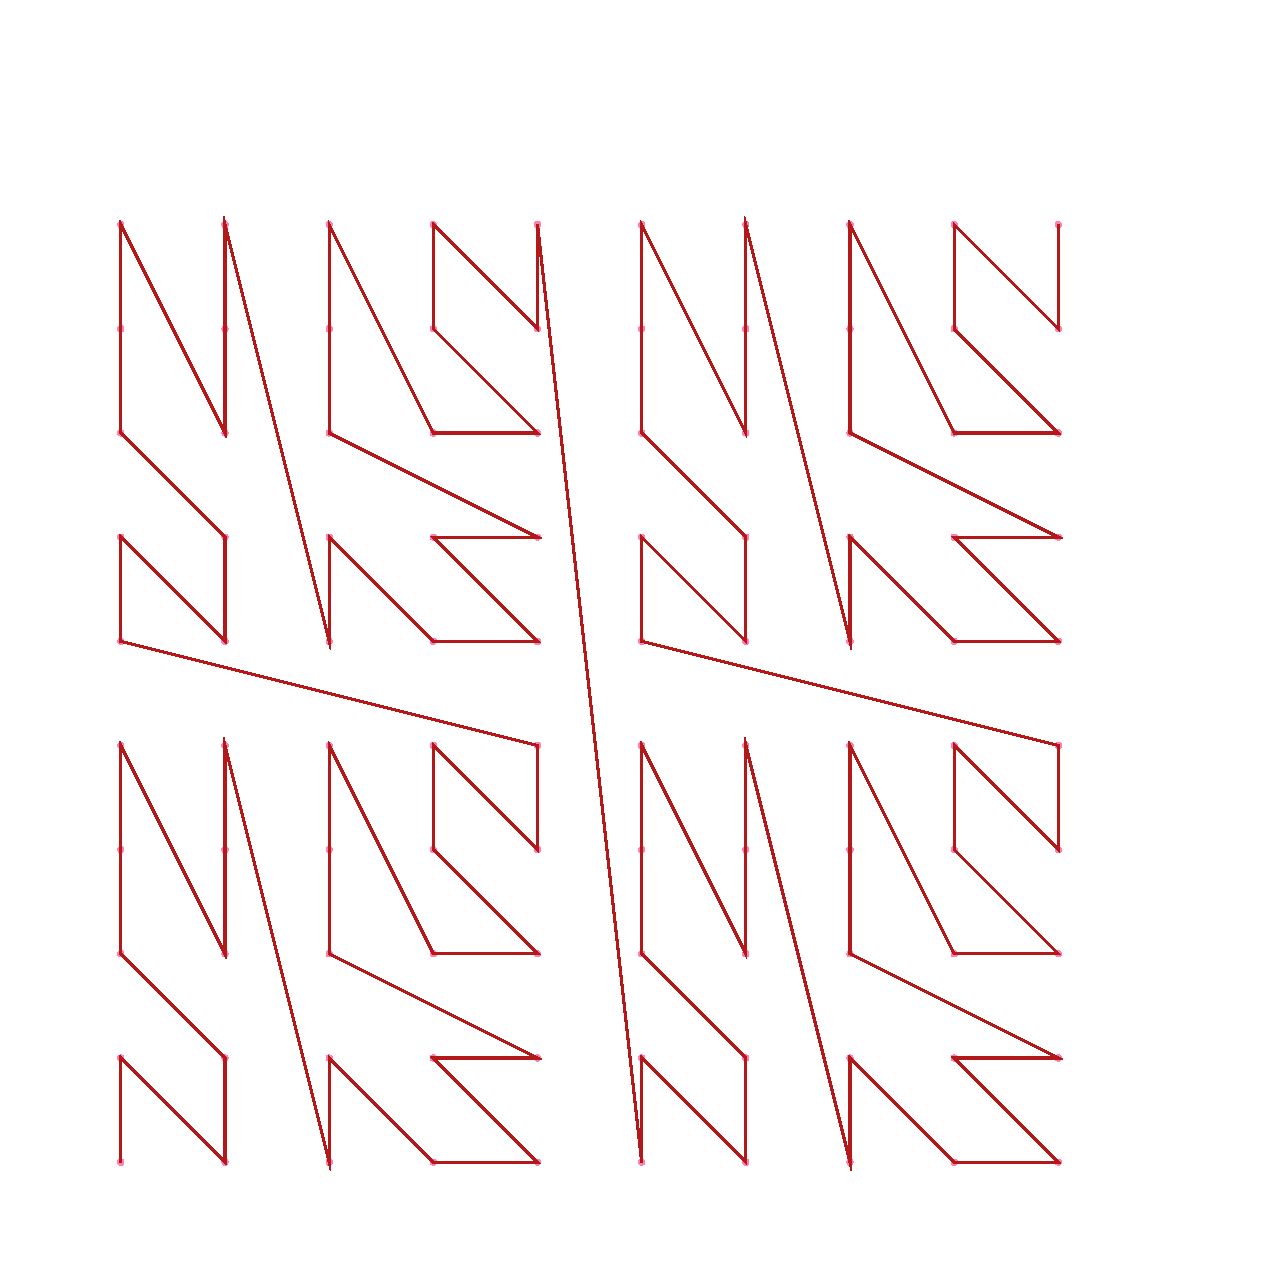
\includegraphics[scale=0.4]{diagrams/zorder.eps}
\caption{Z-Order}
\end{center}
\end{figure}

The points are then sorting according their shuffle order. Each two adjacent
points in the sorted order form a node in the quadtree, which can then be
nested by finding the first larger square to the left and the right in the
sorted order \cite{bern}.

\begin{thm} \emph{(Compressed Quadtree Construction)}
A quadtree containing n points can be constructed in \(O(n log n)\) time
\cite{bern}.
\end{thm}

Chan \cite{chan} showed that the shuffle can be calculated without explicitly
interleaving the bits, and \cite{connor} showed that this can be extended from
integer values to IEEE-754 floating point values.

TODO: better description of how to build quadtree from sorted points. Better
description of Morton order, space filling curves.

\begin{figure}
\begin{center}
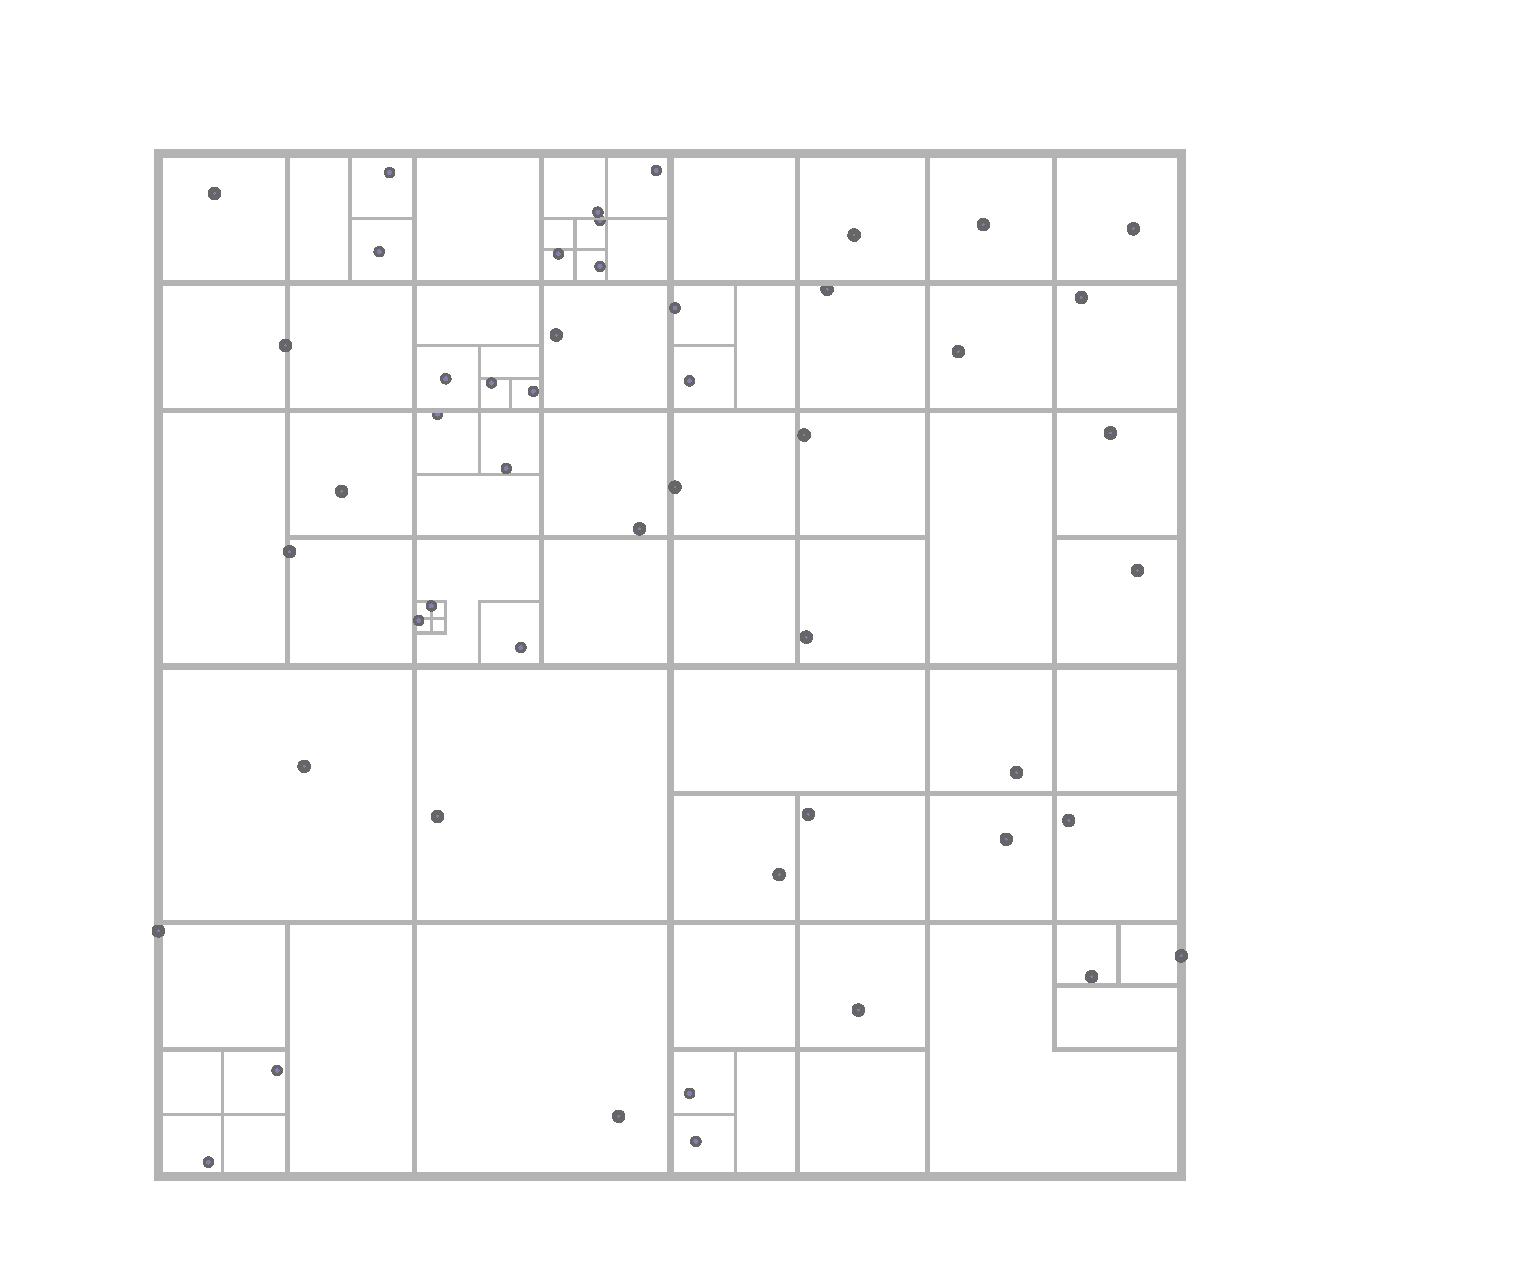
\includegraphics[scale=0.4]{diagrams/compressed_quadtree.eps}
\caption{Compressed Quadtree}
\end{center}
\end{figure}

\begin{thm} \emph{(Height of Compressed Quadtree)}
The height of a compressed quadtree with n points is O(n).
\end{thm}

\subsubsection{Point Location in a Compressed Quadtree}

Point location in a compressed quadtree is done by following the same algorithm
as for standard quadtrees. Since the height of a compressed quadtree is
bounded by the number of points, we can bound the time required to perform
point location.

\begin{thm} \emph{(Point Location in a Compressed Quadtree)} 
Point location in a compressed quadtree with n points can be performed in
time \(O(n)\). 
\end{thm}

\subsubsection{Nearest Neighbour Search in a Compressed Quadtree}

Nearest neighbour search in a compressed quadtree can be done by following the
same algorithm as for standard quadtrees. Again, ince the height of a compressed
quadtree is bounded by the number of points, we can bound the time required to
perform point location.

\begin{thm} \emph{(Nearest Neighbour Search in a Compressed Quadtree)} 
Nearest neighbour search in a compressed quadtree with n points requires
\(O(n)\) time.
\end{thm}

\subsection{Skip Quadtrees}

Skip quadtrees extend the idea of skip lists \cite{skiplist} to 2D and higher
dimensional spaces. In a skip list, multiple levels of linked lists exist, with
pointers between the levels.  The bottom level contains all of the nodes, the
top layer is empty, and (in the randomized version of skip lists,) a node
present in a given layer is present in the layer above it with specified
probability.  Corresponding nodes on different levels are then linked. The
expected number of layers is logarithmic, allowing for search in \(O(\log n)\)
time.

Skip quadtrees use essentially the same idea, except each level is a
compressed quadtree rather than a linked list.

\begin{thm} \emph{(Height of a Quadtree)}
\end{thm}

\begin{thm} \emph{(Quadtree Construction)}
\end{thm}

\subsubsection{Point Location in a Skip Quadtree}

Point location in a skip quadtree is peformed by recursively visiting each level
of the quadtree. Since each level is a compressed quadtree, point location is
first performed in that compressed quadtree. Once the node in the compressed
quadtree is located, the link to the corresponding node in the lower level
is visited until the bottom level is reached and the node in that compressed
quadtree is returned as the result of the point location query.

\begin{thm} \emph{(Point Location in a Skip Quadtree)} 
Point location in a skip quadtree with n points can be performed in time
\(O(log n\)). 
\end{thm}

\subsubsection{Nearest Neighbour Search in a Skip Quadtree}

\begin{thm} \emph{(Nearest Neighbour Search in a Quadtree)} 
Nearest neighbour search in a skip quadtree with n points requires
\end{thm}

\subsection{Kd-Trees}

Kd-trees were described by Jon Bentley in 1975 as an improvement on quadtrees
\cite{kdtree}.  Kd-trees are binary search trees for which each non-leaf node
divides the point set in half using an axis-aligned line.

Kd-trees are constructed by choosing an axis, determining the median value in
the point set for the corresponding coordinate, and dividing the points in two
halves using the median value.  The two child nodes are then built by
recursively building kd-trees for each half.  Depending upon the application,
a number of heuristics exist for choosindg which axis to use for dividing the
points.

\begin{thm} \emph{(Height of a Kd-Tree)}
The height of a kd-tree with n points is O(log n).
\end{thm}

TODO: kd-tree diagram

\subsubsection{Point Location in a Kd-Tree}

\begin{thm} \emph{(Point Location in a Kd-Tree)} 
Point location in a skip quadtree with n points can be performed in time
\(O(n log n\)). 
\end{thm}

\subsubsection{Nearest Neighbour Search in a Skip Quadtree}

Nearest neighbour search in a kd-tree is

\begin{thm} \emph{(Nearest Neighbour Search in a Quadtree)} 
Nearest neighbour search in a kd-tree with n points requires \(O(n)\) time.
\end{thm}

\section{Biased Search}

\subsection{Biased Search Trees}

Biased search trees are a natural generalization of balancing a binary search
tree where rather than assuming each result is equally likely, a probability
distribution is given for the results, allowing the tree to be balanced such
that at each node it is equally likely that the left or right child will be
followed.  The overall expected running time can then be stated in terms of the
entropy of the probability distribution of the queries.

Early work on biased search trees is described in Knuth \cite{knuth} where
the static case (i.e. no deletions and insertions) is considered.  An \(O(n^2)\)
dynamic programming algorithm is presented which constructs an optimum static
search tree for a set of weights.

Biased search trees allowing insertions and deletions based upon 2 - 4 and
red-black trees were described by Bent, Sleator and Tarjan \cite{bst}.  The
data structures are complex and do not appear to have been implemented.
Feigenbaum and Tarjan describe somewhat simpler data structures \cite{bst2}. A
much simpler implementation of biased search based upon randomized search trees
was developed by Aragon and Seidel \cite{treap}, and a biased version of skip
lists \cite{skiplist} was presented in \cite{bsl2}.

An alternative approach to biased search is to use data structures which
modify themselves in response to queries.  In this case, rather than specifying
the probabilities in advance, the data structure will change itself to match
the query distribution.  Splaytrees \cite{splaytree}, which were invented by
Sleator and Tarjan, are a self-modifying binary search tree which have
received considerable attention, both theoretical and experimental due to the
dynamic optimality conjecture, which states that splaytrees are within a
constant factor of optimal for any sequence of queries, without needing to
know the queries in advance.

Most experimental work with biased search has focused on comparing splaytrees
with traditional approaches like 2 - 4 trees and red-black trees.

TODO: give some references on previous experimental work with biased search.

\subsection{Distribution Sensitive Data Structures}

A distribution sensitive data structure has a running time which is a multiple 
of the entropy of the query distribution.  This is similar to biased search
trees, where the running time is given in terms of the entropy of the query
results, but provides a better framework for examining geometric search
problems.

TODO: Explain why better for geometric search.

TODO: Refer to at least Biased Range Trees paper, some results in distribution
sensitive point location.

\subsection{Instance Optimality}

An instance optimal data structure \cite{chan} has a running time which is
within a constant factor of any data structure for any instance of the problem.

TODO: Explain why this gives equivalent results to distribution sensitive data
structures.


\subsection{Odds-on Trees}

TODO: Description of partition tree based odds-on tree.


\chapter{Implementation}

This chapter describes how the odds-on tree was implemented, design decisions
that were made and the performance tuning that was done.

The original description of odds-on trees made use of partition trees.  Although
theoretically optimal, partition trees are not practical to implement, and
implementations were made using both kd-trees and quadtrees.  This chapter
begins with a description of partition tree based odds-on trees, as the
construction and query algorithms are broadly similar to the partition tree
versions.

\section{Kd-tree Implementation}

TODO: brief description of design decisions made during kd-tree implementation,
e.g. point storage, splitting decision, optimizations made.   Refer to 
kd-tree implementation notes in \cite{physicallybasedrendering}.

\section{Kd-tree Based Odds-on Tree}

\subsection{Construction algorithm}

\subsection{Query algorithm}

\section{Quadtree Based Odds-on Tree}

\subsection{Construction algorithm}

TODO: input of m sample points, run NN queries for each point, sort according
to z-order, look for runs in the sort, run interference query, if no
interference, add to cache.  Combine adjacent cache nodes to build bounding
volume hierarchy.

TODO: implement as proper quadtree as well as b.v.h.  same worse case 
performance as compressed quadtree, but may be better in practice?

\subsection{Query algorithm}

TODO: describe query procedure using b.v.h.

\section{Performance Tuning}

TODO: Do some profiling to see if there are any spots which can be optimized. 
TODO: Do experimentation to determine appropriate sample size.
TODO: Do experimentation to determine whether or not it is best to sort by NN
      then by z-order or not.

\chapter{Experimental Results}


\section{Experiment Design}

The experimental hypothesis is that the odds-on tree provides better k-nn
performance than a kd-tree implementation in cases where the entropy of the
query set is sufficiently low.

This hypothesis is tested using both synthetic data drawn from probability
distributions, and with data derived from applications of nearest neighbour
search. 

\subsection{Synthetic Data}

\subsubsection{Dimension}

TODO:
- will definitely experiment in 2, 3, 4 dimensions.
- both kd-trees and quadtrees perform poorly in higher dimensions.  The "curse
of dimensionality" says the number of sample points required to build the cache
should grow quickly as dimension increases, but kd-tree performance also quickly
gets worse.
- will try 8, 16 dimensions in a limited number of cases to see if it is worth
while doing full studies, but literature says this will likely not work well.

\subsubsection{Point Set}

The point set

- distribution of points: uniform or mixture of gaussians
- number of points: 10000, 100000, 1000000 

To reduce variance, the point set which was queried to determine the nearest
neighbour was maintained between trials.  Two distributions were used for the

\subsubsection{Sample Set}

The sample set is the set of searches used to build the odds-on tree.

\subsubsection{Search Set}

The search set is the set of searches used to  test the odds-on tree and
kd-tree implementations.  In all cases, the search set is drawn from the same
distribution used to generate the sample set, and the number of searches was
fixed at 1000000. 

TODO: briefly describe distributions used to generate points: uniform, gaussian,
mixture of gaussians.

\subsection{Application Data}

\subsubsection{Foursquare Dataset}

TODO: describe foursquare dataset, how it is biased, size of dataset, queries
run, etc.

\subsubsection{Photon Mapping Dataset}

Photon mapping is technique used in ray tracing in computer graphics
where lighting is estimated by first creating a photon map by tracing light as
it is emitted from light sources and bounces through the scene, storing the
location each time it hits a surface.  Rays are then traced from the view
location, and each time they hit a surface, the photon map is queried to get an
estimate of the light present at the hit location.  This is a nearest neighbour
search, and it is biased since the queries will only occur on surfaces visible
to the view point, but the photon map will have points for all surfaces visible
to a light source \cite{physicallybased}.

TODO: size of dataset, how to generate a sample dataset, etc.


\section{Measuring Performance}

\subsection{Benchmark Platform}

An Intel Core I5 laptop was used as the benchmark platform.

TODO: Possibly also run experiments on an ARM processor?

\subsection{Performance Metrics}

The primary performance metric is running time.  For each experiment
configuration, 1000000 queries are performed and the elapsed system clock
time is recorded.

In addition to running time, data is collected on the cache miss rate for the
odds-on tree, as well as the number of nodes visited in both the cache and the
back up tree.

Since cache utilization can have a major impact on running time, the Valgrind
\cite{valgrind} cachegrind utility is used to simulate the cache performance
of the implementation, and data is collected on L1 and L2 cache miss rates.

\section{Results}

TODO: one section for each experimental configuration.

\chapter{Conclusion}

\section{Summary}

TODO:

\section{Future Work}

TODO:

\begin{thebibliography}{5}

\bibitem{appnn}
Arya, S., Mount, D. M., Netanyahu, N. S., Silverman, R. Wu, A. Y. (1998) An Optimal Algorithm for Approximate Nearest Neighbor Searching in Fixed Dimensions , Journal of the ACM, Volume 45, Issue 6, 891--923

\bibitem{ann}
Mount, D. M., Arya, S. (2010) ANN: A Library for Approximate Nearest Neighbor Searching, retrieved from \url{http://www.cs.umd.edu/~mount/ANN} on Sept. 27, 2010

\bibitem{chan}
Chan, T. M. (2006) A Minimalist's Implementation of an Approximate Nearest
Neighbour Algorithm in Fixed Dimensions, unpublished note, retrieved from
http://TODO on July X, 2012.

\bibitem{connor}
Connor, M. and Kumar, P. (2009) Fast Construction of k-Nearest Neighbor Graphs
For Point Clouds, IEEE Transactions of Visualizatoin and Computer Graphics,
September 2009.

\bibitem{compressedquadtree}
Clarkson, Kenneth L. (1983) Fast Algorithms for the All Nearest Neighbors Problem,
FOCS '83: Proceedings of the Twenty-fourth Symposium on Foundations of Computer Science,
Tucson, AZ 

\bibitem{dutch}
de Berg., M. van Kreveld, M., Overmars, M., Schwarzkopf, O. (2000)
Computational Geometry: Algorithms and Applications, 2nd Edition, Springer-Verlag,
Berlin Heidelberg New York

\bibitem{kdtree}
Bentley, J. L. (1975) Multidimensional Binary Search Trees Used for Associative Searching,
In Communications of the ACM, Volume 18, Number 9, pp. 509--517 

\bibitem{treap}
Aragon, C. R.,  Seidel, R. (1996) Randomized Search Trees.
In Algorithmica, Vol. 16, Number 4/5, pp. 464 – 497

\bibitem{skipquadtree}
Eppstein, D., Goodrich, M. T., Sun, J. Z. (2008) The Skip Quadtree: A Simple Dynamic Data Structure for Multidimensional Data, Int. Journal on Computational Geometry and Applications, 18(1/2), 131--160 

\bibitem{bsl}
Bagchi,A. Buchsbaum, A. L., Goodrich, M. T. (2005) Biased Skip Lists.
In Algorithmica Vol. 42, pp. 31 – 48

\bibitem{chazelle} Chazelle, B. (1993) Cutting hyperplanes for divide-and-conquer.
Discrete and Compututational Geometry 9, pp. 145--158.

\bibitem{splaytree}
Sleator, D. D., Tarjan, R. E. (1985) Self-adjusting binary search trees.
In Journal of the ACM, 32, pp. 652 – 686

\bibitem{knuth}
Knuth, D. E. (1998) The Art of Computer Programming, Second Edition,
Volume 3, Sorting and Searching.  Addison-Wesley, Reading, Massachusetts, USA.

\bibitem{bsl2}
Ergun, F., Sahinalp, S. C., Sharp, J., Sinha, R. K. (2001) Biased Skip Lists
for Highly Skewed Access Patterns, Proceedings of ALENEX 2001, Lecture Notes in
Computer Science, Volume 2153, 216-229 

\bibitem{bst}
Bent, S. W., Sleator, D. D., Tarjan, R. E. (1984) Biased Search Trees,
In SIAM Journal on Computing, Volume 14, pp. 545 - 568

\bibitem{bst2}
Feigenbaum, J., Tarjan, R. E. (1983) Two New Kinds of Biased Search Tree,
In Bell Systems Technical Journal, Vol. 62, No. 10, pp. 3139 - 3158

\bibitem{kirkpatrick}
Kirkpatrick, D. (1983) Optimal Search in Planara Subdivisons,
Siam Journal of Computing, Vol. 12, No. 1, pp 28 -- 34.

\bibitem{practicalann}
Liu, T., Moore, A. W., Gray, A., Yang, K. (TODO) An Investigation of Practical
Approximate Nearest-Neighbour Algorithms, TODO

\bibitem{quadtree}
Finkel, R. A. and Bentley, J. L. (1974) Quad Trees A Data Structure for
Retrieval on Composite Keys
Acta Informatica, 4(1), pp. 1 – 9 

\bibitem{rtree}
Guttman, A. (1984) R-Trees: A Dynamic Index Structure for Spatial Searching,
TODO 

\bibitem{skiplist}
Pugh, W. (1990) Skip Lists: A Probabilistic Alternative to Balanced Trees.
In Communications of the ACM, 33(6), pp. 668 – 676

\bibitem{samet}
Samet, H. (2006) Foundations of Multidimensional and Metric Data Structures
Morgan-Kaufmann, San Francisco, CA.

\bibitem{satp}
Williams, H. E., Zobel, J., Heinz, S. (2001) Self-Adjusting Trees in Practice
for Large Text Collections, In Software - Practice and Experience,
Volume 31, pp. 925 - 939

\bibitem{valgrind}
Nethercote, N., Seward, J. (2007) Valgrind: A Framework for Heavyweight Dynamic
Binary Instrumentation.  Proceedings of ACM SIGPLAN 2007 Conference on
Programming Language Design and Implementation (PLDI 2007),
San Diego, California, USA

\end{thebibliography}

\end{document}
